\documentclass{article}

\usepackage[german]{babel}
\usepackage{array}
\usepackage[letterpaper,top=2cm,bottom=2cm,left=3cm,right=3cm,marginparwidth=1.75cm]{geometry}

\usepackage{amsmath}
\usepackage{graphicx}
\usepackage{subcaption} % Added package
\usepackage[colorlinks=true, allcolors=blue]{hyperref}
\usepackage[T1]{fontenc}
\usepackage{tabularx}
\usepackage{booktabs}


\title{Übungsprotokoll - NWG2 - Übung 05 \\ Link Aggregation}
\author{\vspace{0.5cm} Thomas Brandstetter (s2210239002) \& Jakob Mayr (s2210239021)}

\begin{document}
\maketitle

\section{Konfiguration der Endsysteme}

In der folgenden Übung haben wir die PCs 4.1 und 4.2 benutzt, somit sind die Netze 4.x verwendet worden. Die IP-Konfiguration wird folgendermaßen vergeben: Klick auf „Network“ in der Taskleiste $\rightarrow$ „Network \& Internet Settings“ $\rightarrow$ „Change adapter options“ $\rightarrow$ gewünschtes Netzwerk Interface auswählen, in diesem Fall Ethernet 2 $\rightarrow$ „Properties“ $\rightarrow$ Doppelklick auf „Internet Protocol Version 4“ bzw. „Internet Protocol Version 6“. In den geöffneten Fenstern können wir nun jeweils die IP-Adresse, Subnetzmaske/Präfix und das Gateway eingeben. Folglich sind die Konfigurationen beider PCs zu sehen:

\begin{figure}[!htp]
  \centering
  \begin{minipage}[b]{0.2\textwidth}
    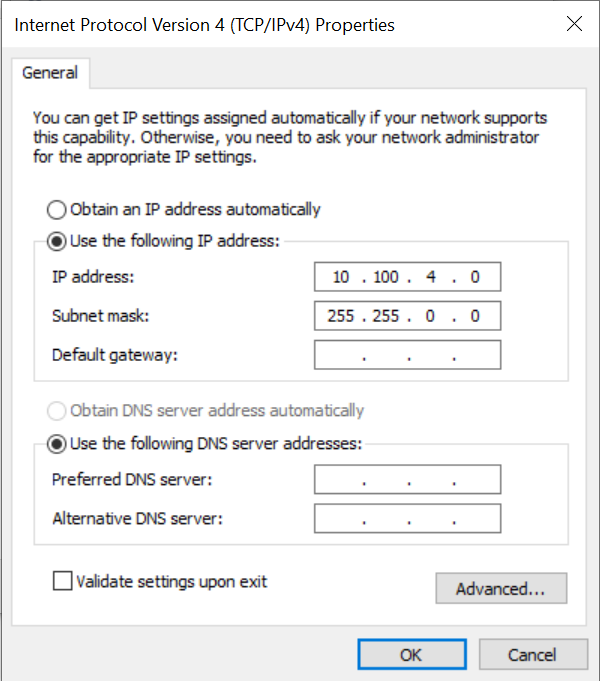
\includegraphics[width=\textwidth]{Arbeitsergebnisse/PC41/pc41_IPv4_config.png}
    \caption{PC41 IPv4 config}
  \end{minipage}
  \hspace{0.8cm}
  \begin{minipage}[b]{0.2\textwidth}
    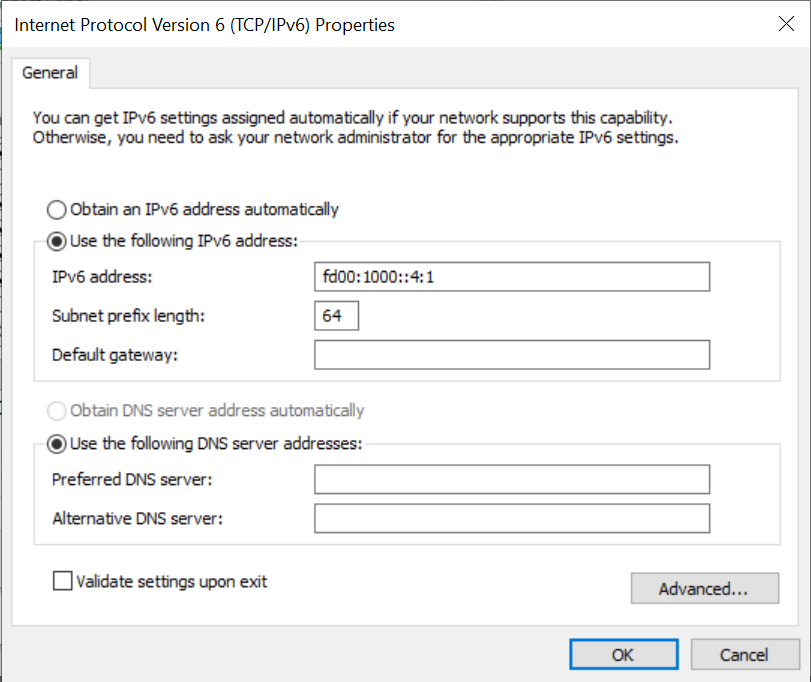
\includegraphics[width=\textwidth]{Arbeitsergebnisse/PC41/pc41_IPv6_config.png}
    \caption{PC41 IPv6 config}
  \end{minipage}
  \hspace{0.8cm}
  \begin{minipage}[b]{0.2\textwidth}
    \includegraphics[width=\textwidth]{Arbeitsergebnisse/PC42/pc42_IPv4_config.png}
    \caption{PC42 IPv4 config}
  \end{minipage}
  \hspace{0.8cm}
  \begin{minipage}[b]{0.2\textwidth}
    \includegraphics[width=\textwidth]{Arbeitsergebnisse/PC42/pc42_IPv6_config.png}
    \caption{PC42 IPv6 config}
  \end{minipage}
\end{figure}

\pagebreak



\section{Konfiguration des Gruppenrouters}

Für die Konfiguration des Gruppenrouters müssen die Interfaces GigabitEthernet0/0 und GigabitEthernet0/1 mit einer IPv4 und einer IPv6 Adressen versehen werden. Ebenfalls muss dafür ipv6-unicast-routing aktiviert werden.\\
Als Default-Gateway wird sowohl für IPv4 als auch für IPv6 der Backbone-Router angegeben.\\


\begin{table}[htbp]
    \centering
    \begin{tabularx}{\textwidth}{|X|X|}
        \toprule
        \textbf{Befehl} & \textbf{Erklärung} \\
        \midrule
        ip address <ip-address> <ip-address-mask> & Mit diesem Befehl wird auf einem Interface eine IPv4 Adresse mit der zugehörigen Maske konfiguriert.\\
        \hline
        ipv6 address <ipv6-address/ipv6-address-mask> & Mit diesem Befehl wird auf einem Interface eine IPv6 Adresse mit der zugehörigen Maske konfiguriert.\\
        \hline
        ip route <network-number> <network-mask> <ip-address|interface> & Mit diesem Befehl wird eine statische IPv4 Route angelegt.\\
        \hline
        ipv6 route <network-number/network-mask> <ipv6-address|interface> & Mit diesem Befehl wird eine statische IPv6 Route angelegt.\\
        \hline
        ipv6-unicast-routing & Mit diesem Befehl wird das unicast-routing für IPv6 aktiviert.\\
        \bottomrule
    \end{tabularx}
    \caption{Verwendete Befehle zur Konfiguration des Gruppenrouters}
\end{table}

\noindent Als nächstes müssen auf dem Router die notwendigen ACLs (access-control-lists) konfiguriert werden.\\
Hierfür soll sowohl jeder eingehende Trafik von den PCx1's zu PC41, als auch jeder eingehende ICMP Trafik zu PC42 geblockt werden.\\
Für die ACL der linken PCs werden die Adressen der PCx1's einzeln in einer IPv4 und einer IPv6 ACL geblockt.\\
Für die ACL des rechten PCs wird jeder ICMP Trafik geblockt.\\

\begin{table}[htbp]
    \centering
    \begin{tabularx}{\textwidth}{|X|X|}
        \toprule
        \textbf{Befehl} & \textbf{Erklärung} \\
        \midrule
        ip access-list extended <ACL-name> & Mit diesem Befehl wird eine ACL für IPv4 angelegt.\\
        \hline
        ipv6 access-list extended <ACL-name> & Mit diesem Befehl wird eine ACL für IPv6 angelegt.\\
        \hline
        deny ip host <src-ip-address> host <dest-ip-address> & Mit diesem Befehl wird der Trafik von der src-ip-Adresse zur dest-ip-Adresse geblockt.\\ 
        \hline
        deny ipv6 host <src-ipv6-address> host <dest-ipv6-address> & Mit diesem Befehl wird der Trafik von der src-ipv6-Adresse zur dest-ipv6-Adresse geblockt.\\
        \hline
        deny icmp host <ipv4/ipv6-address> any & Mit diesem Befehl wird jeder eingehende icmp auf die angegebene Adresse geblockt.\\
        \hline
        permit ip any any / ipv6 permit any any & Diese Befehle müssen am Ende einer ACL hinzugefügt werden, da die Regeln Schritt-für-Schritt abgearbeitet werden und Trafik per-default geblockt wird. Nur mit dieser Regel wird der Trafik welcher von keiner vorherigen Regel geblockt oder speziell erlaubt wird durchgelassen.\\ 
        \bottomrule
    \end{tabularx}
    \caption{Verwendete Befehle zum anlegen der ACLs}
    \label{tab:commands}
\end{table}

\noindent Damit die ACLs nun auch vom Router verwendet werden können, müssen sie noch den jeweiligen Interfaces hinzugefügt werden.\\

\begin{table}[htbp]
    \centering
    \begin{tabularx}{\textwidth}{|X|X|}
        \toprule
        \textbf{Befehl} & \textbf{Erklärung} \\
        \midrule
        ip access-group <ACL-name> in & Mit diesem Befehl wird eine IPv4-ACL einem Interface hinzugefügt.\\
        \hline
        ipv6 traffic-filter <ACL-name> in & Mit diesem Befehl wird eine IPv6-ACL einem Interface hinzugefügt.\\
        \bottomrule
    \end{tabularx}
    \caption{Verwendete Befehle zum hinzufügen der ACLs zu den Interfaces.}
    \label{tab:commands}
\end{table}

\pagebreak

\section{Konfiguration der Gruppenswitches}

Für die Konfiguration der Gruppenswitches ist eine Link-Aggregation zu konfigurieren.\\
Hierzu müssen zuerst auf beiden Switches ein Port-Channel (1) mit dem load-balancing-mode angelegt werden. Anschließend müssen auf den jeweiligen Interfaces das channel-protocol (lacp) und die channel-group (1) im mode aktiv angelegt werden.\\

\begin{table}[htbp]
    \centering
    \begin{tabularx}{\textwidth}{|X|X|}
        \toprule
        \textbf{Befehl} & \textbf{Erklärung} \\
        \midrule
        port-channel load-balance <load-balancind-mode> & Mit diesem Befehl wird ein Port-Channel mit dem jeweiligen load-balancing-mode konfiguriert. (Für diese Aufgabe funktioniert der „src-dst-ip“ mode, da bei diesem der Trafik der beiden Clients klar von einander getrennt werden kann. Anders könnte der Trafik nicht auf zwei Interfaces aufgeteilt werden.)\\
        \hline
        channel-protocol <protocol> & Mit diesem Befehl wird auf dem jeweiligen Interface das channel-protocol spezifiziert. (Für diese Aufgabe das lacp - link aggregation control protocol.)\\
        \hline
        channel-group <number> mode <aktiv/passive> & Mit diesem Befehl wird auf dem jeweiligen Interface die channel-group in dem spezifizierten Modus konfiguriert.\\
        \bottomrule
    \end{tabularx}
    \caption{Verwendete Befehle zur Konfiguration der Gruppenswitches (Link-Aggregation)}
    \label{tab:commands}
\end{table}

\subsection{Mirror-Port}

Zuletzt soll auf dem Gruppenswitch GS41 noch ein Mirror-Port eingerichtet werden. Dieser soll als Eingangsport den Port-Channel der zuvor konfigurierten Channel-Group und als Ausgangsport den Port an dem der linke PC41 hängt haben.

\begin{table}[htbp]
    \centering
    \begin{tabularx}{\textwidth}{|X|X|}
        \toprule
        \textbf{Befehl} & \textbf{Erklärung} \\
        \midrule
        monitor session <number> source interface <interface-name> & Mit diesem Befehl wird der Eingangsport für den Mirror-Port bestimmt.\\
        \hline
        monitor session <number> destination interface <interface-name> & Mit diesem Befehl wird der Ausgangsport für den Mirror-Port bestimmt.\\
        \bottomrule
    \end{tabularx}
    \caption{Verwendete Befehle zur Konfiguration des Mirror-Ports}
    \label{tab:commands}
\end{table}


\section{Fragen zur Konfiguration}

\subsection*{Frage 5.1 \normalfont Warum können ohne die Link Aggregation (das Erstellen der Channel Group) nicht beide Links verwendet werden?}
Ohne Link Aggregation, auch bekannt als Port Trunking oder EtherChannel, würden die beiden parallelen Fast Ethernet Verbindungen als separate, unabhängige Links betrachtet werden. Dies kann zu mehreren Problemen führen:
\begin{itemize}
  \item Ungleichmäßige Lastverteilung: Ohne Link Aggregation wäre es schwierig, den Datenverkehr gleichmäßig über die beiden Links zu verteilen. In der Regel würde ein Switch den Datenverkehr über einen Link senden, bis dieser voll ist, und dann erst den anderen Link verwenden. Dies führt zu einer ineffizienten Nutzung der verfügbaren Bandbreite.\\

  \item Fehlende Redundanz und Ausfallsicherheit: Ohne Link Aggregation, wenn ein Link ausfällt, würde der Datenverkehr, der über diesen Link fließt, unterbrochen werden, bis der Switch den Ausfall erkennt und auf den anderen Link umschaltet. Mit Link Aggregation würde der Datenverkehr einfach über den verbleibenden Link weitergeleitet werden, wenn ein Link ausfällt, was zu einer höheren Ausfallsicherheit führt.\\
\end{itemize}

\subsection*{Frage 5.2 \normalfont Wie kann durch ein geeignetes Load Balancing sichergestellt werden, dass beide Rechner mit voller Geschwindigkeit bedient werden?}
Dies kann erreicht werden, indem man beispielsweise das Load Balancing so konfiguriert, dass es auf der Basis der Quell- und Ziel-IP-Adressen und/oder Portnummern arbeitet. Auf diese Weise würde der Verkehr von und zu den beiden verschiedenen Rechnern wahrscheinlich auf die beiden verschiedenen Links verteilt werden, was dazu beitragen würde, dass beide Rechner mit voller Geschwindigkeit bedient werden.\\

\subsection*{Frage 5.3 \normalfont Wenn Gruppe A die ACLs bereits fertig konfiguriert hat, Gruppe B aber nicht, wie wirkt sich das auf Ping zwischen den linken PCs aus? Falls es nicht geht, welche Fehlermeldungen erscheinen wann?}

\begin{itemize}
  \item Gruppe B bekommt ein „Destination Host Unreachable“, da der Router von Gruppe A den Trafik blockiert.
  \item Gruppe A kann normal pingen da keine ACL dies verhindert und bekommt somit einen erfolgreichen Ping-Echo.
\end{itemize}
\subsection*{Frage 5.4 \normalfont Wie wirken sich die ACLs auf den Kontakt zum FTP Server aus, und warum?} 
Da die ACL einerseits den Trafik von anderen Clients (PCx1) und andererseits ICMP Trafik sperren, haben sie keine Auswirkung auf den Kontakt zum FTP Server. Wichtig ist dafür jedoch die „permit ip any any“ regel am Ende der ACL.\\

\pagebreak

\subsection*{Frage 5.5 \normalfont Was bedeutet es für den linken PC, dass er an einem Mirror Port hängt? Wie wirkt sich das auf seine Kommunikationsfähigkeit aus? Welche ports sollten für einen Mirror Port verwendet werden und warum?}
Wenn der linke PC an einem Mirror Port hängt, bedeutet das, dass er eine Kopie des Netzwerkverkehrs von den Quellports empfängt. Dies sollte seine normale Kommunikationsfähigkeit nicht beeinflussen - er kann immer noch Netzwerkverkehr senden und empfangen wie gewohnt. Der Unterschied ist, dass er zusätzlich eine Kopie des Netzwerkverkehrs von den Quellports empfängt.\\

\noindent In Bezug auf die Auswahl der Ports für einen Mirror Port, sollte der Mirror Port in der Regel an einen dedizierten Überwachungs- oder Analysegerät angeschlossen werden, wie z.B. einen PC mit Netzwerkanalyse-Software (wie Wireshark). Der Quellport (oder die Quellports) sollte derjenige sein, dessen Verkehr Sie überwachen oder analysieren möchten. Es ist wichtig zu beachten, dass der Mirror Port nur eine Kopie des Verkehrs empfängt - er kann nicht auf diesen Verkehr antworten oder interagieren. Daher ist es in der Regel nicht sinnvoll, einen Mirror Port für normale Netzwerkkommunikation zu verwenden.\\

\pagebreak
\section{Tests und Interpretation ihrer Resultate}

\subsection{GS41 \& GS42}
Verwendete „Load-Balancing“ Konfiguration auf des Switchtes GS41 und GS42:\\
\begin{figure}[!htp]
  \centering
  \begin{minipage}[b]{0.45\textwidth}
    \includegraphics[width=\textwidth]{Arbeitsergebnisse/GS41/GS41_etherchannel.png}
    \caption{GS41 EtherChannel Load-Balancing Configuration}
  \end{minipage}
  \hspace{0.8cm}
  \begin{minipage}[b]{0.45\textwidth}
    \includegraphics[width=\textwidth]{Arbeitsergebnisse/GS41/GS41_etherchannel.png}
    \caption{GS41 EtherChannel Load-Balancing Configuration}
  \end{minipage}
\end{figure}

\pagebreak
\subsection{PC41}
Ping von PC41 zu PC42, Ping zu Netz 8 - PC81 (fehlgeschlagen da ACL) und FTP-Verbindung\\
\begin{figure}[!htp]
  \centering
  \begin{minipage}[b]{0.25\textwidth}
    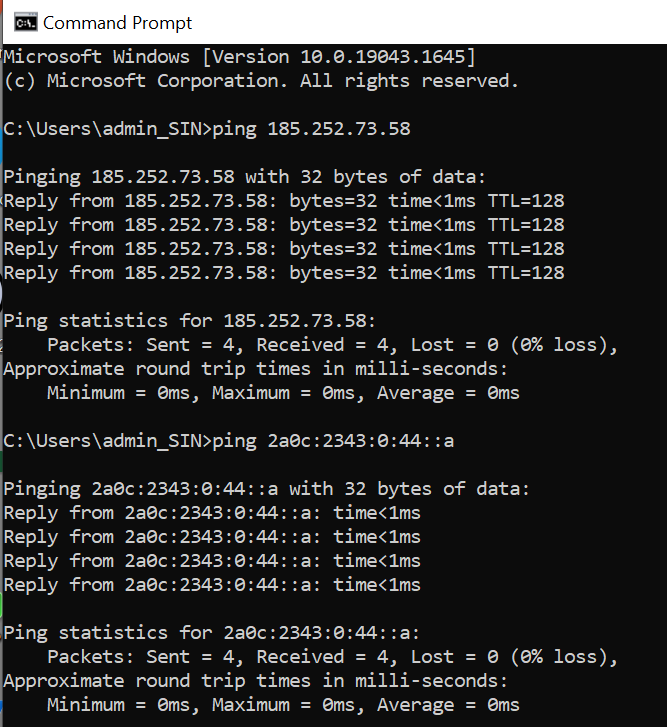
\includegraphics[width=\textwidth]{Arbeitsergebnisse/PC41/pc41_ping_pc42.png}
    \caption{PC41 ping PC42}
  \end{minipage}
  \hspace{0.8cm}
  \begin{minipage}[b]{0.25\textwidth}
    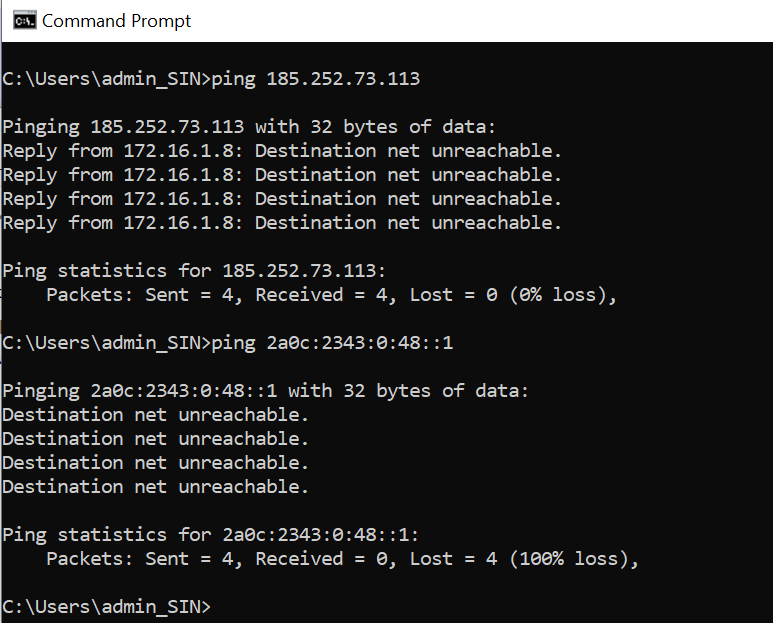
\includegraphics[width=\textwidth]{Arbeitsergebnisse/PC41/pc41_ping_failed.png}
    \caption{PC41 Ping zu Netz 8 - PC81 (fehlgeschlagen da ACL)}
    Dieser fehlgeschlagene ping zum Gruppenrouter von Gruppe 8 zeigt, dass die ACL von Gruppe 8 korrekt umgesetzt wurde.\\
  \end{minipage}
  \hspace{0.8cm}
  \begin{minipage}[b]{0.25\textwidth}
    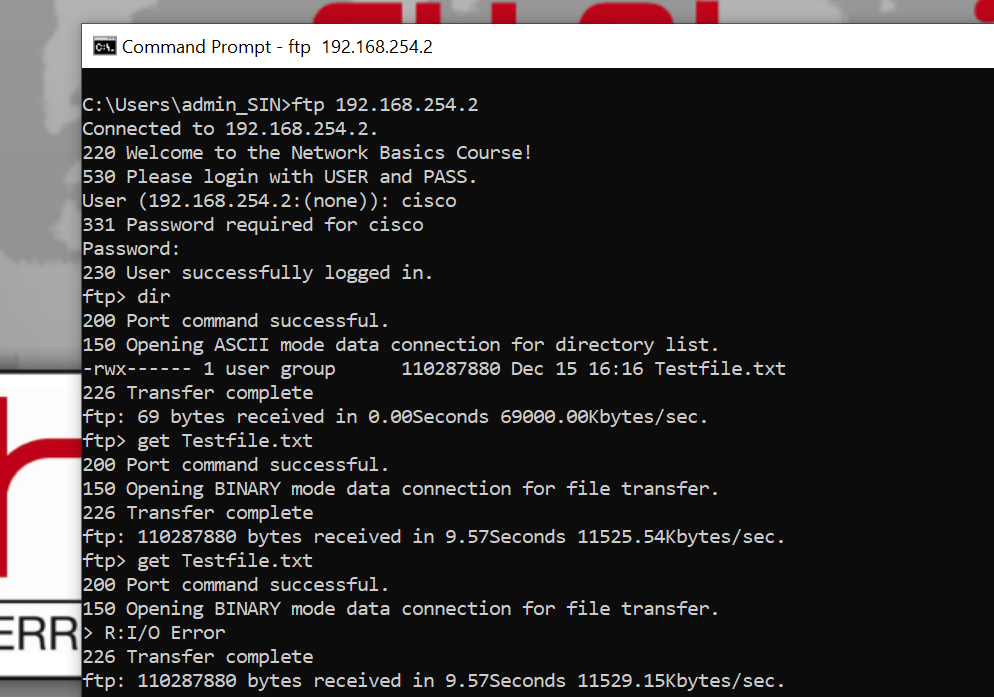
\includegraphics[width=\textwidth]{Arbeitsergebnisse/PC41/pc41_ftp.png}
    \caption{PC41 FTP-Verbindung}
  \end{minipage}
\end{figure}

\subsection{PC42}
Ping von PC42 zu PC41, Ping zu Netz 8 - PC82 (fehlgeschlagen da ACL) und FTP-Verbindung\\
\begin{figure}[!htp]
  \centering
  \begin{minipage}[b]{0.25\textwidth}
    \includegraphics[width=\textwidth]{Arbeitsergebnisse/PC42/pc42_ping_PC41.png}
    \caption{PC42 ping PC41}
  \end{minipage}
  \hspace{0.8cm}
  \begin{minipage}[b]{0.25\textwidth}
    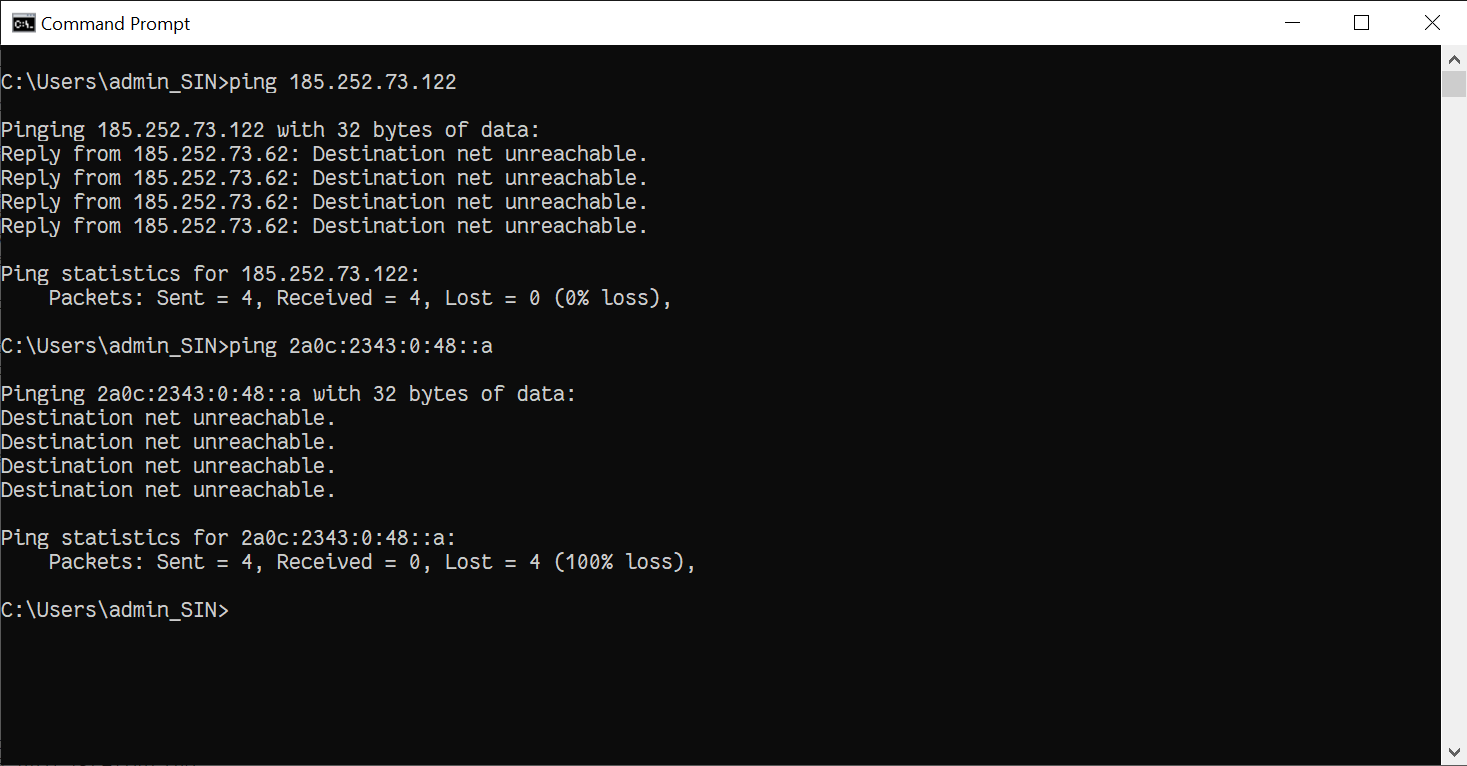
\includegraphics[width=\textwidth]{Arbeitsergebnisse/PC42/pc42_ping_failed.png}
    \caption{PC42 Ping zu Netz 8 - PC82 (fehlgeschlagen da ACL)}
    Dieser fehlgeschlagene Ping zu PC82 zeigt, dass die ACL von Gruppe 8 korrekt umgesetzt wurde.\\
  \end{minipage}
  \hspace{0.8cm}
  \begin{minipage}[b]{0.25\textwidth}
    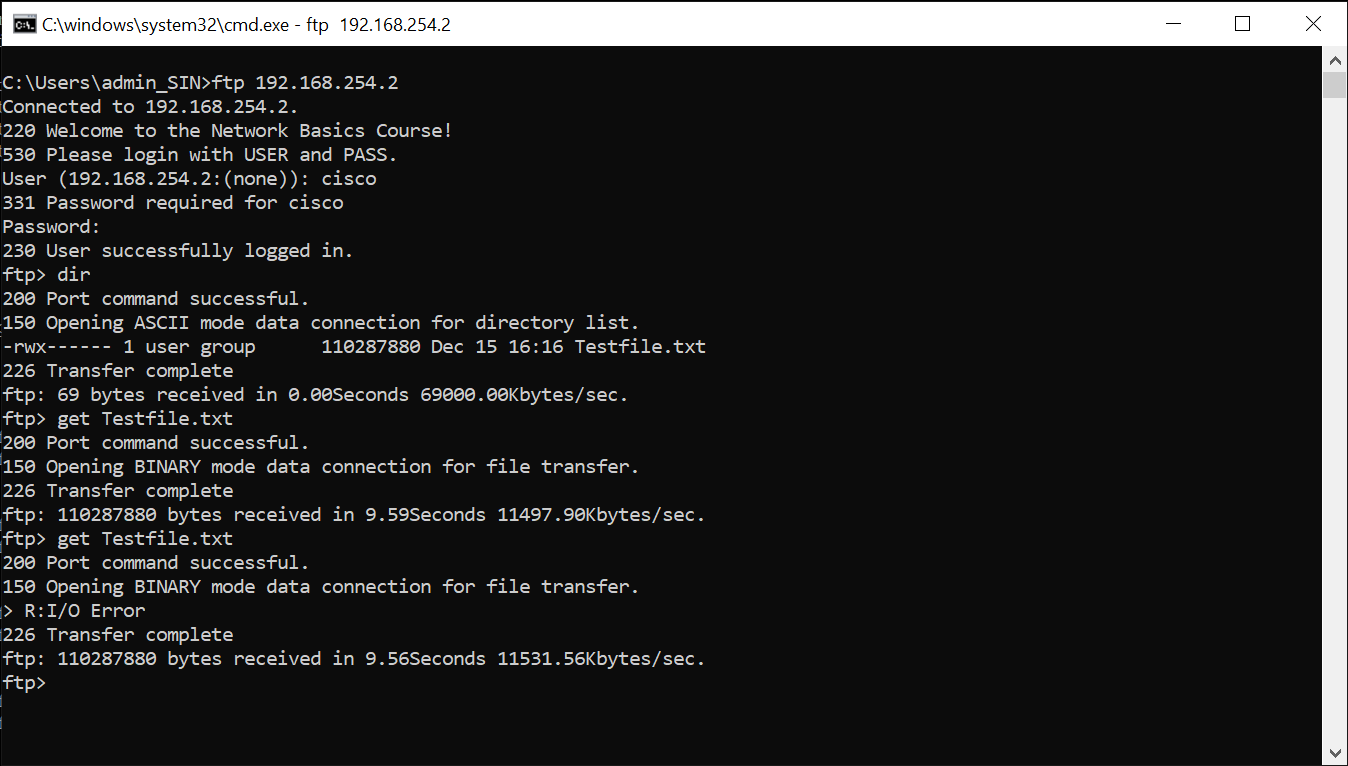
\includegraphics[width=\textwidth]{Arbeitsergebnisse/PC42/pc42_ftp.png}
    \caption{PC42 FTP-Verbindung}
  \end{minipage}
\end{figure}

\end{document}

